\documentclass{beamer}
%
% Choose how your presentation looks.
%
% For more themes, color themes and font themes, see:
% http://deic.uab.es/~iblanes/beamer_gallery/index_by_theme.html
%
\mode<presentation>
{
  \usetheme{default}      % or try Darmstadt, Madrid, Warsaw, ...
  \usecolortheme{default} % or try albatross, beaver, crane, ...
  \usefonttheme{default}  % or try serif, structurebold, ...
  \setbeamertemplate{navigation symbols}{}
  \setbeamertemplate{caption}[numbered]
} 

\usepackage[english]{babel}
\usepackage[export]{adjustbox}
 % \usepackage[utf8x]{inputenc}
\usepackage[style=authoryear]{biblatex}
\addbibresource{references.bib}
\usepackage{tikz}
\graphicspath{{figures/}}
\DeclareMathOperator{\sign}{sign}

\usepackage{caption}
\captionsetup{font=scriptsize, labelfont=scriptsize}

\newcommand{\specialcell}[2][c]{%
  \begin{tabular}[#1]{@{}c@{}}#2\end{tabular}}

\title[Your Short Title]{Qualifying Exam: Examples of my approach and research}
\author{Adam Massmann}
\date{December 7th, 2017}

\begin{document}

\begin{frame}
  \titlepage
\end{frame}


\section{Introduction}
\begin{frame}{Current project - When does vapor pressure deficit (VPD) drive or reduce evapotranspiration (ET)?}
  \begin{columns}[T,onlytextwidth]
    \begin{column}{0.5\textwidth}
      \begin{minipage}{\textwidth}
        \begin{itemize}
        \item A \textbf{hydrometeorologist} might say that an increase in VPD (increase in \textbf{atmospheric demand}) would drive an \textbf{increase in ET}.
        \item However, \textbf{plant physiologists} know that plants have evolved to use stomata to conserve and regulate water use. So \textbf{stomata closure} in response to increases in VPD may \textbf{decrease ET}.
        \end{itemize}
      \end{minipage}
    \end{column}
    \begin{column}{0.5\textwidth}
      \begin{minipage}{\textwidth}
        \begin{figure}
          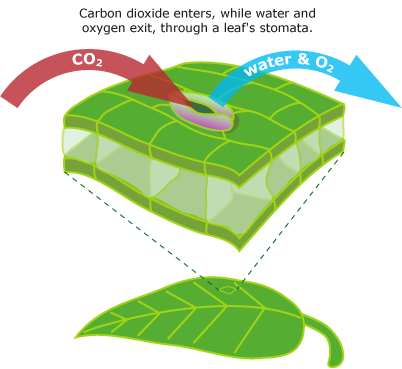
\includegraphics[width=2.00in]{stomata.png}% was O(1.5in)
          \caption{from evolution.berkeley.edu}
        \end{figure}
      \end{minipage}
    \end{column}
  \end{columns}
\end{frame}

\section{Method}

\begin{frame}{My approach}
  \begin{itemize}
  \item Use physically reasonable assumptions guided by intuition and literature to simplify the problem and develop a transparent and intuitive theory (or hypothesis). The goal is to capture the leading order behavior of the system.
    \begin{itemize}
    \item Here we start with Penman Monteith, and apply an assumption of constant uWUE (recently identified by \cite{Zhou_2016}) which gives a differentiable function of ET.
    \end{itemize}
  \item Test theory with observational or sophisticated model data to see if theory is valid, and to what extent it may generalize.
    \begin{itemize}
    \item Here we use FLUXNET2015 data.
    \end{itemize}
  \end{itemize}
\end{frame}

\section{Results - theory}
\begin{frame}{Results - theory's form for ET response to VPD perturbations}
  \begin{tikzpicture}
    \node[anchor=south west,inner sep=0] (image) at (0,0) {\adjincludegraphics[width=3.5in, trim={0 {0.51\height} 0 0}, clip]{fig05.pdf}};
        \begin{scope}[x={(image.south east)},y={(image.north west)}]
        %% next four lines will help you to locate the point needed by forming a grid. comment these four lines in the final picture.↓
       % \draw[help lines,xstep=.1,ystep=.1] (0,0) grid (1,1);
       % \draw[help lines,xstep=.05,ystep=.05] (0,0) grid (1,1);
       % \foreach \x in {0,1,...,9} { \node [anchor=north] at (\x/10,0) {0.\x}; }
       % \foreach \y in {0,1,...,9} { \node [anchor=east] at (0,\y/10) {0.\y};}
       %% upto here
        \draw[-latex, line width=2pt] (0.83,0.725) --++(0.0in,0.3in)node[anchor=south] {ET Increasing};
        \draw[-latex, line width=2pt] (0.83,0.725) --++(0.0in,-0.3in)node[anchor=north] {ET Decreasing};

        % \draw[dashed,-latex, line width=5pt] (0.8,0.75) --++(0.0in,+0.5in)node[anchor=north] {ET Decreasing};
    \end{scope}
    % \node[align=center,red,font={\large}] at (image.southwest) {ET decreasing};
  \end{tikzpicture}
\end{frame}


\section{Test Theory}
\begin{frame}{Testing Theory - the good: evergreen forest}
  \includegraphics[width=3.5in]{enf_eee.png}
\end{frame}

\begin{frame}{Testing Theory - the bad: grassland}
  \includegraphics[width=3.5in]{gra_eee.png}
\end{frame}

\section{Conclusions}

\begin{frame}{Summary - When does VPD reduce ET?}
  \small
  \begin{itemize}
  \item Successfully simplified the problem to develop a theory for when atmospheric dryness will increase ET (atmospheric demand dominates) vs. decrease ET (plant response dominates).
  \item Tested the theory with real data from FLUXNET2015: shrubs and forests tested well, while the theory's applicability to crops and grass is more uncertain.
  \item All plant types except for crops has a common occurrence of decreases in ET with increases in VPD (plant response dominates). Therefore, any drought indices which assume that atmospheric demand dominates (e.g PET-based metrics) are likely unrealistic for vegetated surfaces.
  \end{itemize}
\end{frame}

\section{References}
\begin{frame}{References}
  \AtNextBibliography{\small}
  \printbibliography
  \scriptsize
  \begin{itemize}
  \item This work used eddy covariance data acquired and shared by the FLUXNET community, including these networks: AmeriFlux, AfriFlux, AsiaFlux, CarboAfrica, CarboEuropeIP, CarboItaly, CarboMont, ChinaFlux, Fluxnet-Canada, GreenGrass, ICOS, KoFlux, LBA, NECC, OzFlux-TERN, TCOS-Siberia, and USCCC. The ERA-Interim reanalysis data are provided by ECMWF and processed by LSCE. The FLUXNET eddy covariance data processing and harmonization was carried out by the European Fluxes Database Cluster, AmeriFlux Management Project, and Fluxdata project of FLUXNET, with the support of CDIAC and ICOS Ecosystem Thematic Center, and the OzFlux, ChinaFlux and AsiaFlux offices.
    \item This material is based upon work supported by the National Science Foundation Graduate Research Fellowship under Grant No. DGE 16-44869. Any opinion, findings, and conclusions or recommendations expressed in this material are those of the authors(s) and do not necessarily reflect the views of the National Science Foundation.
    \end{itemize}
\end{frame}

\section{Extra Slides}

    \begin{frame}{Test theory with FLUXNET data - CSH}
                \includegraphics[width=3.5in]{csh_eee.png}
     \end{frame}


    \begin{frame}{Test theory with FLUXNET data - DBF}
                \includegraphics[width=3.5in]{dbf_eee.png}
     \end{frame}

    \begin{frame}{Test theory with FLUXNET data - CRO}
                \includegraphics[width=3.5in]{cro_eee.png}
     \end{frame}

\begin{frame}{Extra slide - statistics}
  \begin{table}
  \label{vpd_crit}
\caption{More quantitative test of theory.}
\centering
\begin{tabular}{l c c c c c c}
  \hline
  PFT & \specialcell{Fraction of Obs.\\Theory is Correct} & Mean ($\frac{\partial \; ET}{\partial \; VPD} < 0$) & Mean ($\frac{\partial \; ET}{\partial \; VPD} > 0$)\\
  \hline
  CRO & 0.566517 & -0.209152 &  0.005856\\
  CSH & 0.931660 & -0.264746 &       NaN\\
  DBF & 0.633363 & -0.135679 &  0.042910\\
  ENF & 0.633138 & -0.150665 &  0.029281\\
  GRA & 0.442306 & -0.042158 & -0.042480\\
  \hline
\end{tabular}
\end{table}
\end{frame}

\begin{frame}{Extra slide - is theory VPD$_{crit}$ optimum?}
  \includegraphics[width=\textwidth]{for_agu.pdf}
\end{frame}

% \begin{frame}{Summary statistics - extra sl}
%      \begin{table}
%        \caption{Statistics of $\frac{\partial \; ET}{\partial \, VPD}$ as a function of PFT.}
%        \centering
%        \begin{tabular}{l c c}
%          \hline
%          PFT & $\overline{\frac{\partial \; ET}{\partial \; VPD}}$ & fraction $\frac{\partial \; ET}{\partial \; VPD} < 0.$ \\
%          \hline
%          CRO & 0.000853  & 0.473311\\
%          CSH & -0.108234 & 0.931660\\
%          DBF & -0.012727 & 0.461674\\
%          ENF & -0.034087 & 0.534425\\
%          GRA & -0.019637 & 0.631735\\
%          \hline
%          \multicolumn{2}{l}{}  
%        \end{tabular}
%      \end{table}
%    \end{frame}
     




% \begin{table}
% \centering
% \begin{tabular}{l|r}
% Item & Quantity \\\hline
% Widgets & 42 \\
% Gadgets & 13
% \end{tabular}
% \caption{\label{tab:widgets}An example table.}
% \end{table}

\end{document}
